\documentclass[output=paper,colorlinks,citecolor=brown
% ,hidelinks
% showindex
]{langscibook}
\author{Guy Tabachnick\orcid{0009-0006-5705-516X}\affiliation{Masaryk University}}
% \author{}
% REPLACE THE ABOVE WITH YOU AND YOUR CO-AUTHORS, YOUR AFFILIATIONS, AND YOUR ORCID NUMBERS
% rules for affiliation: If there's an official English version, use that (find out on the official website of the university); if not, use the original
% orcid doesn't appear printed; it's metainformation used for later indexing

\SetupAffiliations{mark style=none}
% comment in (i.e. remove the % sign at the beginning of the line) the above line if you are a single author or all authors have the same affiliation

% \lehead{Šimík, Gehrke, Lenertová, Meyer, Szucsich \& Zaleska}
% in case the running head with authors exceeds one line (which is the case in this example document), use one the above method to turn it into a single line; otherwise comment the line above out with % and ignore it

\title[Russian speakers use inflectional knowledge in choosing nonce words]{Russian speakers use inflectional knowledge in choosing the diminutive of nonce words}
% REPLACE THE ABOVE WITH YOUR PAPER TITLE
% provide a shorter version of your title in case it doesn't fit a single line in the running head
% in this form: \title[short title]{full title}

\abstract{Russian masculine nouns may take a number of diminutive suffixes, and Russian speakers follow a number of gradient statistical generalizations over nouns' phonological properties in deciding which diminutive to assign to existing and novel words \citep{Polivanova2008,Gouskova.etal2015}. In a corpus study, I show that Russian diminutive allomorphy is also sensitive to two morphological properties: a noun's inflectional stress pattern and its plural suffix. Moreover, speakers productively extend these generalizations alongside the phonological ones in a nonce word study. I propose that speakers store these generalizations in the form of gradient constraints over the cooccurrence of morphological markers on underlying forms. This has implications for morphological theory: theories of allomorphy must be flexible enough to allow words to have two independently varying inflectional markers accessible to one and the same pattern-matching module.

\keywords{frequency matching, productivity, morpheme structure constraints, nonce word study, morphology, Russian}
}

\input{localpackages.tex}
\makeatletter
\let\thetitle\@title
\let\theauthor\@author 
\makeatother

\newcommand{\togglepaper}[1][0]{ 
%   \bibliography{../localbibliography}
  \papernote{\scriptsize\normalfont
    \ResolveAffiliations
      [output affiliation=false, output authors font=\normalfont]
      {\theauthor}.
    \titleTemp. 
    To appear in: 
    Change Volume Editor \& in localcommands.tex 
    Change volume title in localcommands.tex
    Berlin: Language Science Press. [preliminary page numbering]
  } 
  \pagenumbering{roman}
  \setcounter{chapter}{#1}
  \addtocounter{chapter}{-1}
}

% add commmands of your own if needed
\newcommand{\mC}[1]{\multicolumn{1}{c}{#1}} % multicolumn with a single column

\newcommand\pla{[á]}
\newcommand\pli{[i]}
\newcommand\plsi{[í]}
\newcommand\ok{[ók]}
\newcommand\ik{[ʲik]}
\newcommand\chik{[tʃʲik]}

\newcommand{\DIM}{\textsc{dim}{}\xspace}	%diminutive

\newcommand\gap{\_\_\_}

\newcommand{\feat}[2][\textit]{[#1{#2}]}
\newcommand{\urfeat}[3][\textit]{/#2\textsubscript{\feat[#1]{#3}}/}

\setlength{\unitlength}{1em}
\newcommand\like[1]{\begin{picture}(1,1)
 \ifnum0=#1\put(.5,.35){\circle{1}}\else
 \ifnum10=#1\put(.5,.35){\circle*{1}}\else
 \put(.5,.35){\circle{1}}\put(.5,.35){\circle*{.#1}}
\fi\fi\end{picture}
}

\hyphenation{par-a-digms}

% for formatting percent sign in tables
\ExplSyntaxOn
\NewDocumentCommand \tabpct {}
  {
    \siunitx_unit_format:nN {\percent} \l_tmpa_tl
    \siunitx_quantity_print:nV { } \l_tmpa_tl
  }
\ExplSyntaxOff

% keep this here (at the end of this document)
\AtBeginDocument{\nogltOffset} %removes extra spacing before trans line in examples

\bibliography{localbibliography}

\IfFileExists{../localcommands.tex}{
   \addbibresource{../localbibliography.bib}
   \input{../localpackages}
   \makeatletter
\let\thetitle\@title
\let\theauthor\@author 
\makeatother

\newcommand{\togglepaper}[1][0]{ 
%   \bibliography{../localbibliography}
  \papernote{\scriptsize\normalfont
    \ResolveAffiliations
      [output affiliation=false, output authors font=\normalfont]
      {\theauthor}.
    \titleTemp. 
    To appear in: 
    Change Volume Editor \& in localcommands.tex 
    Change volume title in localcommands.tex
    Berlin: Language Science Press. [preliminary page numbering]
  } 
  \pagenumbering{roman}
  \setcounter{chapter}{#1}
  \addtocounter{chapter}{-1}
}

% add commmands of your own if needed
\newcommand{\mC}[1]{\multicolumn{1}{c}{#1}} % multicolumn with a single column

\newcommand\pla{[á]}
\newcommand\pli{[i]}
\newcommand\plsi{[í]}
\newcommand\ok{[ók]}
\newcommand\ik{[ʲik]}
\newcommand\chik{[tʃʲik]}

\newcommand{\DIM}{\textsc{dim}{}\xspace}	%diminutive

\newcommand\gap{\_\_\_}

\newcommand{\feat}[2][\textit]{[#1{#2}]}
\newcommand{\urfeat}[3][\textit]{/#2\textsubscript{\feat[#1]{#3}}/}

\setlength{\unitlength}{1em}
\newcommand\like[1]{\begin{picture}(1,1)
 \ifnum0=#1\put(.5,.35){\circle{1}}\else
 \ifnum10=#1\put(.5,.35){\circle*{1}}\else
 \put(.5,.35){\circle{1}}\put(.5,.35){\circle*{.#1}}
\fi\fi\end{picture}
}

\hyphenation{par-a-digms}

% for formatting percent sign in tables
\ExplSyntaxOn
\NewDocumentCommand \tabpct {}
  {
    \siunitx_unit_format:nN {\percent} \l_tmpa_tl
    \siunitx_quantity_print:nV { } \l_tmpa_tl
  }
\ExplSyntaxOff

% keep this here (at the end of this document)
\AtBeginDocument{\nogltOffset} %removes extra spacing before trans line in examples

   \input{../localhyphenation}
   \boolfalse{bookcompile}
}{}

\togglepaper[42]
%the chapter number will be provided by volume editors; for now keep this way


%%%% TO DO
% recode with animates

%%%% CITATION QUESTIONS
% Polivanova, Zaliznyak, corpus: full name or initials?
% Polivanova, corpus: original Russian or official English translation?
% Melvold date


\begin{document}
\maketitle

% \input{template-osl.tex}
% Just comment out the line above (place % at its beginning) and start writing your own document
% WRITE DIRECTLY HERE, INTO main.tex, DO NOT START YOUR OWN tex FILE!

% START WRITING HERE

\section{Introduction}\label{sec:intro}

Russian has a number of productive diminutive suffixes that attach to nouns of various genders and inflection classes \citep[cf.][]{Steriopolo2008}. % and others
This study focuses on three diminutive suffixes that attach with some level of productivity to the main inflectional class of masculine nouns \citep[class I according to][]{Corbett1982}: \ok, \ik, and \chik. In general, a given noun may be attested with one or more of these suffixes. Russian speakers have to learn which suffixes go with which words, and previous studies show that they have learned numerous statistical correlations between nouns' phonological properties and the diminutive suffixes they combine with \citep{Gouskova.etal2015, Magomedova2017}.

I present the results of corpus and experimental studies showing that Russian speakers have also learned \emph{morphological} generalizations over diminutive selection: \ok{} is preferred by nouns that have stressed suffixes in some or all of their inflectional paradigm, and in particular, by nouns with the stressed plural suffix \pla{}. I argue that speakers learn these correlations as cooccurrence relations over properties of underlying forms: if a noun's underlying form has the ``inflectional suffix stress'' property and the ``takes plural \pla'' property, it is also likely to have the ``takes diminutive \ok'' property, but these three are formally independent. Thus, any theory of grammar that attempts to encode inflection class or other selectional properties through pieces of phonology or syntax must satisfy two criteria: first, lexical items may have multiple such pieces that independently covary, and second, these pieces must be accessible within the same % really?
pattern-matching module -- which, I propose, is phonological. % work on this

% recode with animates!!

\section{Background}\label{sec:bg}
\subsection{Diminutives}\label{sec:dimbg}
The three diminutives discussed in this paper are shown in \tabref{tab:dimex}.\footnote{Unless otherwise noted, I ignore the reduction of unstressed vowels.}
% no velar-final examples with final stress?
\begin{table}
% \begin{tabularx}{.45\textwidth}{llX}
\begin{tabular}{llll}
\lsptoprule
% noun & diminutive & gloss\\
& `novel' & `package' & `staff'\\
\midrule
% román & román-tʃʲik & `novel'\\
% pakʲét & pakʲét-ʲik & `package'\\
% pósox & posoʂ-ók & `staff'\\
base & román & pakʲét & pósox\\
diminutive & romántʃʲik & pakʲétʲik & posoʂók\\
\lspbottomrule
% \end{tabularx}
\end{tabular}
\caption{Examples of Russian masculine nouns and their diminutives}
\label{tab:dimex}
\end{table}
This table demonstrates two morphophonological properties of \ok{} (neither of which are unique to it): first, \ok{} triggers an alternation in stem-final velars like [x] \citep[see][]{Kapatsinski2010,Magomedova.Slioussar2017}. Second, \ok{} is always stressed in the nominative singular; following \citet{Melvold1989}, it is dominant -- it erases any lexical accent on its base -- and post-accenting -- it bears lexical accent that is realized on inflectional suffixes. The vowel in the suffix is also ``fleeting'' (as is common for Russian mid vowels); that is, it disappears when further suffixes are attached. Thus, the genitive singular of [posoʂók] from \tabref{tab:dimex} is [posoʂká].

\citet{Polivanova2008} identifies a number of phonological generalizations describing a given noun's choice of diminutive: for example, nouns ending in clusters always take \ik{}, velar-final nouns select \ok{}, and \chik{} and \ik{} only attach to nouns with final stress. \citet{Gouskova.etal2015} confirm many of these tendencies in an elicitation study, though their findings are often not as categorical as \citet{Polivanova2008} had claimed. They also find several additional gradient tendencies in a corpus study of the Russian lexicon, some of which are productively used by speakers in a nonce word study. Thus, for example, nouns ending in sonorants rarely end in \ik{}, and Russian speakers are hesitant to choose \ik{} for sonorant-final nonce words, accordingly.

% \citet{Magomedova2017} argues for a semantic distinction between the diminutives: in words that accept both \ok{} and \ik, the latter is more affectionate, while the former is somewhat more pejorative (both of these shades of meaning are typical for diminutives). % Likewise, speakers assigned \ik{} more often to nonce words given an affectionate meaning and preferred \ok{} to those presented in a pejorative context.
\citet{Magomedova.Slioussar2017} argue that the three suffixes are not entirely competing allomorphs: % reword
they claim that \ok{} is somewhat less productive than \ik{} and \chik{} due to its phonological properties and the fact that speakers are reluctant to extend it to loanwords \citep[see][]{Gouskova.etal2015,Magomedova2017}. In this study, however, I argue that previous studies have overlooked contexts in which \ok{} is as productive as the other suffixes. Similarly, \citet{Magomedova2017} argues that the suffixes show some semantic differentiation as well: \ik{} tends to be used more often in affectionate contexts, while \ok{} is preferred in pejorative contexts. However, this distinction is incomplete (she thus calls the suffixes pseudo-allomorphs): \ik{} and \ok{} are frequently used for both real and nonce words with both affectionate and pejorative meaning. % in this paper...

\subsection{Inflectional stress}\label{sec:strbg}
As mentioned above, \ok{} diminutives have stress fixed on inflectional suffixes. Russian nouns may follow this or a number of other inflectional stress patterns, as shown in \tabref{tab:inflex}. Of these, fixed stem stress is by far the most common, while mobile stress is the rarest for masculine nouns. Other mobile stress patterns (that is, where a different set of suffixes is stressed) are more common in other inflection classes \citep{Brown.etal1996}.
% not sure I like the justification/arrangement here
\begin{table}
% \begin{tabularx}{.45\textwidth}{llX}
\begin{tabular}{l@{ }llll}
\lsptoprule
% noun & diminutive & gloss\\
&& `bus' & `pencil' & `hair'\\
\midrule
\SG{} & \NOM{} & avtóbus & karandáʂ & vólos\\
\SG{} & \DAT{} & avtóbusu & karandaʂú & vólosu\\
\PL{} & \NOM{} & avtóbusɨ & karandaʂɨ́ & vólosɨ\\
\PL{} & \DAT{} & avtóbusam & karandaʂám & volosám\\[.5ex]
\multicolumn{2}{l}{stress} & stem & suffix & mobile\\
\lspbottomrule
% \end{tabularx}
\end{tabular}
\caption{Examples of inflectional stress patterns in Russian masculine nouns}
\label{tab:inflex}
\end{table}

Many generative analyses \citep[e.g.][]{Melvold1989,Halle1997,Revithiadou1999} % good mix?
derive the differences between the stress patterns in \tabref{tab:inflex} \citep[see also][166--8]{Molczanow.etal2013} from differences in underlying accent and the Basic Accentuation Principle \citep{Kiparsky.Halle1977}, which states that stress falls on the leftmost accented syllable or, if there is no underlying accent, on the first syllable. Thus, fixed stem stress is lexical (/avtóbus/), nouns with fixed suffix stress (known as post-accenting) have a lexical accent that falls onto the next syllable (/karandaʂ´/), and nouns with mobile stress are underlyingly accentless (/volos/). For such nouns, stress falls on the suffix if it has a lexical accent and on the first syllable of the word if it does not (in which case both stem and suffix are accentless). Thus, for this inflection class, dative plural /ám/ is accented (as are other oblique plural suffixes), while the nominative plural of [vólosɨ] (/i/) and singular suffixes like dative /u/ are not.

\subsection{Plural}\label{sec:plbg}
There is some variation in the nominative plural of masculine nouns. Most nouns have [ɨ$\sim$i] (the alternation is phonologically conditioned), which is unstressed for mobile-stress nouns like [vólos], and thus, following the Basic Accentuation Principle, underlyingly. A larger group of monosyllabic nouns, like [nos] `nose', has stress throughout the plural, including in the nominative ([nosɨ́]).

Another group of masculine nouns, like [kólokol] `bell', has [a] in the nominative plural (the typical ending for neuter nouns) and suffix stress throughout the plural ([kolokolá]). The use of this plural is dialectally and sociolinguistically conditioned, though standard dictionaries list approximately 250 nouns in this class \citep{Worth1983}. Most of these nouns have stem stress throughout the singular, so they are typically classed as mobile-stress nouns. However, unlike most words with mobile stress, these nouns do not necessarily have initial stress in stem-stressed forms as predicted by the Basic Accentuation Principle. \citet{Shapiro1985} notes that (with some scant exceptions) masculine nouns with plural \pla{} have \emph{non-final} stress in the singular, which, for longer words like [utʃʲítʲelʲ] `teacher' (plural [utʃʲitʲelʲá]), may be medial. Thus, the representation of (at least some) plural \pla{} nouns must differ from typical underlyingly unaccented mobile stress nouns. % move this later?

\subsection{Correlations between forms}
As mentioned in \sectref{sec:dimbg}, previous studies have investigated the phonological properties correlated with a noun's choice of diminutive and shown that speakers have learned these correlations from their lexicon. These studies belong to a line of cross-linguistic research finding that speakers are sensitive to correlations between the phonological shape of words and the lexically specific morphological processes they undergo \citep[e.g.][]{Albright.Hayes2003,Becker2009,Hayes.etal2009,Becker.etal2011}.

The present study looks at another type of generalization: correlations between affixed forms with the same base. Speakers of morphologically complex languages encounter only a small percentage of possible forms of most words in their lexicon \citep{Chan2008}, yet are typically able to generate these previously unseen forms when needed. Thus, they must have some way of inferring unknown members of a word's inflectional paradigm from known members. In some cases, this inference is relatively straightforward -- for example, in Russian, knowing one or two of a noun's forms is typically enough to figure out its inflection class (that is, the set of inflectional suffixes it takes) and its stress pattern \citep[though there are complexities in this inference process that are often ignored; see][]{Parker.Sims2020}. Indeed, morphological systems seem to be organized in a way that facilitates these inferences between cells, and an active line in morphological research has studied this implicative paradigm structure \citep[e.g.][]{Wurzel1989,Ackerman.etal2009,Ackerman.Malouf2013,Bonami.Beniamine2016}.

However, very few studies have actually demonstrated experimentally how (or even that) speakers actually use known forms to infer unknown ones. The nonce word studies of \citet{Copot.Bonami2023} and \citet{Tabachnick2024} show that speakers productively extend correlations between paradigm cells to nonce words in French and Hungarian, respectively. The present study adds to this burgeoning line of research by demonstrating that Russian speakers likewise extend lexical correlations between paradigm cells in nonce words. First, in \sectref{sec:corp}, I show that the diminutive of Russian nouns is correlated with two properties of its inflectional paradigm: its inflectional stress pattern and its plural suffix. In \sectref{sec:exp}, I then show that Russian speakers have productively learned these correlations and use them to infer the diminutive of nonce words from their plural.

\section{Corpus study}\label{sec:corp}
As described in \sectref{sec:dimbg}, previous studies of the Russian lexicon have shown that a noun's phonology is partially predictive of its choice of diminutive. This corpus study replicates many of these previous findings using a new source, the Russian National Corpus, and also provides novel evidence for another feature of a Russian noun correlated with its diminutive: its \emph{inflectional morphology}. In particular, I show that nouns with some or all stressed suffixes in their inflectional paradigm are more likely to take the diminutive \ok, and nouns with plural \pla{} are more likely still to take \ok{} than other nouns with mobile stress.

\subsection{Design and hypotheses}\label{sec:corphyp}
The corpus study was originally intended to test the hypothesis (developed from ancedotal observation) that nouns with plural \pla{} prefer diminutive \ok. Given that \pla{} is associated with particular inflectional stress patterns, this had to be accounted for in the analysis. The correlation between \ok{} and inflectional stress, though clear in the data, was not the original target of analysis.

Similar to \citet{Gouskova.etal2015}, I modelled the effects of each diminutive suffix. The models predicting use of \ik{} and \chik, although they contained the same factors, are more exploratory in nature and not relevant to the present study; thus, I do not present them here.

\subsection{Data}\label{sec:corpdata}
I look at nouns from the main masculine inflection class according to inflectional data from \citet{Zaliznjak1977}, which specifies endings and stress patterns. I exclude words with more than one listed inflectional pattern or stress location, words listed as mass nouns (which have no plural), and words with one of three stem extensions: plural [j] (e.g.\ [klʲin] `wedge', nominative plural [klʲínʲja]), singular [ʲin] (e.g. [ɡraʐdanʲín], nominative plural [ɡráʐdanʲe]), and singular [ʲón(o)k] alternating with plural [ʲát] (e.g. [tʲelʲónok] `calf', nominative plural [tʲelʲáta].

I then constructed possible diminutives for each noun, taking into account regular and semi-regular morphophonological alternations. Thus, as described in \sectref{sec:dimbg}, \ok{} palatalizes velars, so [posoʂók] was included as a possible diminutive of [pósox] `staff' but [posoxók] was not. Nouns ending in velars almost never take \ik{}, so it is unclear whether this diminutive suffix triggers velar palatalization as well \citep[see][]{Kapatsinski2010,Magomedova.Slioussar2017}; in my data, however, potential diminutives with \ik{} after non-alternating velars were false positives (e.g.\ [lóɡʲik] `logic' is not the diminutive of [loɡ] `ravine'), so I likewise only included potential \ik{} diminutives with palatalized velars: [pósoʂɨk], not [pósoxik].\footnote{Although it is itself the outcome of a palatalization alternation, Russian [ʂ] patterns as a hard (unpalatalized) consonant phonologically, meaning that /i/ following [ʂ] surfaces as [ɨ].} This diminutive also typically causes an alternation of [ts] to [tʃʲ], so a word like [abzáts] `indentation' had potential diminutives [abzátsɨk] and [abzátʃʲik] (exceptionally, in this case the diminutive is attested with [ts]). Similarly, \chik{}, as a rule, palatalizes [l], so [orʲólʲtʃʲik] was tested as a diminutive of [orʲól] `eagle' alongside [orʲóltʃʲik] (forms like the latter appear very rarely, if ever). Finally, \ik{} often but not always triggers a vowel--zero alternation for words that have one in their inflectional pattern. Thus, [xrʲebʲét] `ridge' (genitive singular [xrʲebʲtá]) has potential diminutives [xrʲebʲétʲik] and [xrʲébʲtʲik] (both of which are attested).

Next, I searched for all forms of lemmas for both base nouns and constructed diminutives in texts of the main corpus of the Russian National Corpus \citep{Savchuk.etal2024} % cite better?
written after 1950 (its cutoff for modern written texts). This corpus is easy to access and includes a wide range of genres of written texts. As it is intended to represent the modern standard language, its use of diminutives and other neologisms is likely somewhat more conservative than one would find in a web-based corpus. Nonetheless, it includes a wide range of diminutives and seems sufficiently representative for the present purposes.

While the Russian National Corpus is much larger and better tagged than the source of data used by \citet{Gouskova.etal2015} in their corpus study, it does have two main sources of false positive diminutives. The first is that forms are sometimes mistagged -- accordingly, I manually filtered out tokens whose endings did not match the expected case endings. Second, there are ``pseudo-diminutives'' that are orthographically identical to expected combinations of base and diminutive but do not have the intended meaning. The main source of these is homographic suffixes, such as in [alkoɡólʲik] `alcoholic', which is not the diminutive of [alkoɡólʲ] `alcohol', and [pulʲemʲóttʃʲik] `machine gun operator', which is not the diminutive of [pulʲemʲót] `machine gun' \citep[cf.][]{Gouskova.etal2015,GuzmanNaranjo2019}. These suffixes tend to derive animate nouns from inanimate bases, so I removed any diminutives tagged in the corpus with an animacy feature differing from that of its base in the dictionary. More problematic are words ending in \emph{unstressed} [ok], a suffix with numerous uses including an unproductive diminutive (this suffix is written the same as \ok{} in Russian orthography, which does not typically mark stress). For example, the verb [obrʲézatʲ] `trim' has derivatives including [obrʲéz] `edge' and [obrʲézok] `trimming' (usually plural, as in English), but the latter is not the diminutive of the former. In this case, I removed potential diminutives that were themselves listed in \citet{Zaliznjak1977} as ending in unstressed [ok]. Finally, nouns with the suffix [nʲik] (e.g.\ [plavnʲík] `fin') look like diminutives of nouns ending in [(e)nʲ] (e.g.\ [plavʲenʲ] `flux'); I removed all such base--diminutive pairs as well. These measures are altogether fairly effective, though the final data set does include some false positives nonetheless.

After some additional cleanup and removal of infrequent bases (with less than five tokens in the corpus) and bases that were themselves diminutives, my corpus has 12,993 base lemmas, of which 1,409 (\qty{10.8}{\percent}) are attested with at least one diminutive.

\subsection{Methods and analysis}\label{sec:corpanal}
The goal of the corpus study is to establish a correlation between inflectional properties of Russian nouns (primarily, their nominative plural suffix; secondarily, their stress pattern) and diminutive selection. Previous studies, such as \citet{Gouskova.etal2015}, have shown that phonological properties have an effect. Accordingly, I aim to show that these inflectional properties are predictive of diminutive choice even when the phonological factors are taken into account (this study thus constitutes a partial replication of theirs, though the analysis is slightly different).

To do this, I fitted a logistic regression for nouns with at least one attested diminutive predicting whether that noun is attested with diminutive \ok{}. I fitted a forward stepwise regression using the \texttt{buildmer} function from the R package of the same name \citep{RCoreTeam2023,Voeten2023}. This function adds factors to the model one at a time such that each improves the model's Akaike Information Criterion (AIC), which measures both model fit and simplicity (penalizing additional factors). I included among the predictors a range of phonological factors (whether the base was monosyllabic, whether it ended in a cluster, the place and manner of its final consonant, the height and rounding of its last vowel). \citet{Gouskova.etal2015} found an effect of stress location on diminutive suffix, but this is conflated with inflectional stress: nouns with fixed suffix stress have stem-final stress when the stem is unsuffixed, while nouns with mobile stress have stem-initial stress when unsuffixed. Inflectional stress, in turn, is conflated with plural suffix, since all but two nouns with plural \pla{} have mobile stress. % see caveat above
To capture this nesting structure, I combined these three factors into a single factor with five levels (fixed final stem stress, fixed pre-final stem stress, fixed suffix stress, mobile stress with plural \pli, mobile stress with plural \pla) and coded the following contrasts: pre-final vs.\ final stem stress, suffix or mobile vs.\ stem stress, mobile vs.\ suffix stress, and plural \pla{} vs.\ \pli{} mobile stress. Phonological factors were dummy-coded with the most frequent level as the baseline, and all were included in the final model. Terms are listed in the order in which they were added (roughly, by importance).

\subsection{Results}
\subsubsection{Descriptive summary}\label{sec:corpsumm}
\tabref{tab:corpdesc} shows the distribution of the different diminutives according to the inflectional stress patterns and plurals of their bases. The two nouns with suffix stress in the singular that also take plural \pla{} ([rukáv] `sleeve', which appears with \chik, and [obʂláɡ] `cuff', which does not have a diminutive in the corpus) are listed with other suffix-stress nouns.
\begin{table}
\begin{tabular}{lS[table-format = 4.0]S[table-format = 3.0]S[table-format = 3.0]S[table-format = 3.0]S[table-format = 2.0]S[table-format = 2.1{\tabpct}]<{{\tabpct}}}
\lsptoprule
Stress and plural & {none} & {\chik} & {\ik} & {\ok} & {multiple} & \multicolumn{1}{c}{\unit{\percent} \ok}\\
\midrule
final stem & 6159 & 357 & 395 & 65 & 37 & 9.4\\
pre-final stem & 4548 & 5 & 31 & 41 & 4 & 53.7\\
suffix & 788 & 18 & 110 & 208 & 38 & 65.5\\
mobile, \pli & 37 & 0 & 12 & 33 & 13 & 75.9\\
mobile, \pla & 52 & 1 & 2 & 35 & 4 & 92.9\\
\lspbottomrule
\end{tabular}
\caption{Distribution of diminutives in the Russian National Corpus by stress pattern and plural suffix (\unit{percent} [ók] measures the percentage of nouns attested with at least one diminutive that are attested with [ók])} % fix
\label{tab:corpdesc}
\end{table}
Nouns with fixed stem-final stress have a much higher likelihood of not having a diminutive (which is expected given that this is the largest and most productive class), but even when they do, the likelihood that this diminutive is \ok{} is fairly small. Nouns with stress fixed on an earlier stem syllable, which are also quite frequent, have a substantially higher rate of \ok{} Next, in turn, \ok{} is more common still among nouns with suffix stress, and even more so for nouns with mobile stress. Among these, \ok{} is the most prevalent among nouns with plural \pla{}: only a few such nouns allow a diminutive that is not \ok. Thus, both of the inflectional factors (stress pattern and plural suffix) are strongly correlated with the use of diminutive \ok.

\subsubsection{Regression model}
\tabref{tab:corpmod} shows that this correlation between \ok{} and the morphological factors holds even when phonological factors are taken into account: nouns with suffix and mobile stress appear with \ok{} significantly more than those with fixed final stem stress (as do nouns with stress fixed on a non-final syllable); this difference is especially concentrated in nouns with plural \pla, which take \ok{} significantly more than even other nouns with mobile stress.\footnote{Together, the models for \ik{} and \chik{} mentioned in \sectref{sec:corphyp} form the mirror image of the model for \ok{} in \tabref{tab:corpmod}: nouns with mobile stress are significantly less likely to take \ik{} than nouns with suffix stress, while the other three comparisons (pre-final vs.\ final stem stress, suffix/mobile vs.\ stem stress, and mobile with plural \pla{} vs.\ mobile with plural \pli{}) show a significant negative effect for \chik{} (that is, also in the opposite direction from \ok{}).}
% \begin{table}
% \begin{tabular}{l@{~~}lSS[table-format = 0.2, print-zero-integer = false]SS[table-format = +0.4, print-zero-integer = false]@{~~}l}
% \lsptoprule
% \multicolumn{2}{l}{Effect} & {Estimate} & {SE} & {$z$ value} & {$p$ value}\\
% \midrule
% \multicolumn{2}{l}{Intercept} & -2.02 & .26 & -7.69 & <.0001 & ***\\
% \multicolumn{7}{l}{Stress (default: final stem)}\\
% & pre-final stem & 3.38 & .35 & 9.62 & <.0001 & ***\\
% & suffix & 2.25 & .24 & 9.39 & <.0001 & ***\\
% & mobile & 3.24 & .42 & 7.76 & <.0001 & ***\\
% \multicolumn{7}{l}{C place (default: coronal)}\\
% & labial & -.86 & .35 & -2.47 & .0134 & *\\
% & dorsal & 5.37 & .75 & 7.16 & <.0001 & ***\\
% \multicolumn{7}{l}{Length (default: polysyllabic)}\\
% & monosyllabic & 1.83 & .24 & 7.55 & <.0001 & ***\\
% \multicolumn{7}{l}{Coda (default: singleton)}\\
% & cluster & -2.01 & .37 & -5.48 & <.0001 & ***\\
% \multicolumn{7}{l}{Plural (default: \pli)}\\
% & \pla & 2.29 & .70 & 3.25 & .0011 & **\\
% \multicolumn{7}{l}{C Manner (default: plosive)}\\
% & affricate & -1.50 & .48 & -2.15 & .0016 & **\\
% & fricative & -.65 & .31 & -2.07 & .0388 & *\\
% & nasal & -.31 & .30 & -1.04 & .2987\\
% & approximant & .19 & .27 & .68 & .4964\\
% \multicolumn{7}{l}{V height (default: mid)}\\
% & high & .24 & .25 & .98 & .3290\\
% & low & -1.06 & .28 & -3.74 & .0002 & ***\\
% \multicolumn{7}{l}{V rounding (default: unrounded)}\\
% & rounded & -.86 & .24 & -3.66 & .0003 & ***\\
% \lspbottomrule
% \end{tabular}
% \caption{Regression model predicting whether a noun is attested with diminutive [ók]} % fix!
% \label{tab:corpmod}
% \end{table}
\begin{table}
\begin{tabular}{l@{~~}l@{~~}l@{}S@{~~~}S[table-format = 0.2, print-zero-integer = false]@{~~~}S@{~~~}S[table-format = +0.4, print-zero-integer = false]@{~}l}
\lsptoprule
\multicolumn{3}{l}{Effect} & {Estimate} & {SE} & {$z$ value} & {$p$ value}\\
\midrule
\multicolumn{3}{l}{Intercept} & .23 & .32 & .71 & .4755\\
\multicolumn{8}{l}{Stress and plural}\\
& pre-final stem & (vs.\ final stem) & 3.29 & .35 & 9.38 & <.0001 & ***\\
& suffix/mobile & (vs.\ stem) & 1.51 & .21 & 7.23 & <.0001 & ***\\
& mobile & (vs.\ suffix) & 2.15 & .40 & 5.32 & <.0001 & ***\\
& mobile, \pla{} & (vs.\ mobile, \pli) & 2.35 & .75 & 3.16 & .0016 & **\\
\multicolumn{8}{l}{C place}\\ % (default: coronal)}\\
& labial & (vs.\ coronal) & -.35 & .33 & -1.06 & .2923\\
& dorsal & (vs.\ coronal) & 5.59 & .64 & 8.79 & <.0001 & ***\\
\multicolumn{8}{l}{C Manner}\\ % (default: plosive)}\\
& affricate & (vs.\ plosive) & -1.98 & .47 & -4.21 & <.0001 & ***\\
& fricative & (vs.\ plosive) & -.55 & .31 & -1.75 & .0796\\
& nasal & (vs.\ plosive) & .35 & .30 & 1.15 & .2513\\
& approximant & (vs.\ plosive) & .38 & .29 & 1.31 & .1895\\
\multicolumn{8}{l}{Length}\\ % (default: polysyllabic)}\\
& monosyllabic & (vs.\ polysyllabic) & 1.44 & .24 & 6.08 & <.0001 & ***\\
\multicolumn{8}{l}{Coda}\\ % (default: singleton)}\\
& cluster &(vs.\ singleton) & -1.72 & .37 & -4.58 & <.0001 & ***\\
\multicolumn{8}{l}{V rounding}\\ % (default: unrounded)}\\
& rounded & (vs.\ unrounded) & -.91 & .24 & -3.83 & .0001 & ***\\
\multicolumn{8}{l}{V height}\\ % (default: mid)}\\
& high & (vs.\ mid) & .66 & .23 & 2.81 & .0050 & **\\
& low & (vs.\ mid) & -.49 & .27 & -1.79 & .0731\\
\lspbottomrule
\end{tabular}
\caption{Regression model predicting whether a noun is attested with diminutive [ók]} % fix!
\label{tab:corpmod}
\end{table}
The model in \tabref{tab:corpmod} has $R^2=.624$, and multicollinearity between the factors is not a concern: their variance inflation factors (VIF) are between $1.22$ and $1.87$. Each of the phonological factors tested has some effect on the use of \ok. Most saliently, nouns ending in dorsals strongly prefer \ok{}, as do nouns with stress before the final syllable (even after we remove the mobile-stress nouns that fall into this group).

\subsection{Discussion}\label{sec:corpdisc}
In the Russian National Corpus, a noun's choice of diminutive is strongly correlated with two properties of its inflectional paradigm: its stress pattern and its nominative plural. Specifically, nouns with some or all inflectional suffixes stressed appear with \ok{} more often than nouns with stress fixed on the stem (which, in generative analyses, is marked with lexical accent associated with a syllable), and nouns with plural \pla{} appear with \ok{} more often than nouns with plural \pli. In both these cases, \ok, which is post-accenting and which \citet{Magomedova.Slioussar2017} argue to be less productive, clusters with inflectional patterns that are themselves less productive and involve stressed suffixes. % introduce this elsewhere?

\citet{Gouskova.etal2015} looked at a number of phonological factors influencing choice of diminutive, and the present study confirms many of their effects. Least surprisingly, both studies find a strong preference for \ok{} among dorsal nouns compared to coronals (in my study) and all other consonants (in theirs). This effect is near-categorical and is robustly attested in other sources as well \citep{Polivanova2008,Kapatsinski2010,Magomedova.Slioussar2017}. % put more about this in the intro? list the differences between the two studies somewhere?

I replicate the findings of \citet{Gouskova.etal2015} that monosyllabic words take \ok{} more often than longer words (which, they find, prefer \chik) and that words ending in clusters take \ok{} relatively rarely (such words prefer \ik). While they find that words ending in nasals take \ok{} less than obstruent-final nouns, I find a non-significant effect in the opposite direction. I do find that nouns ending in affricates take \ok{} less than those ending in plosives, which \citet{Gouskova.etal2015} likewise did not test for. I do not have a clear explanation for the difference in the nasals -- perhaps the difference lies in the slightly different exclusion criteria between our studies (I used the corpus's lemmatization, their corpus had no morphological analysis; I removed infrequent or variable bases, they did not).

The effect of the vowel in the last syllable of the stem is somewhat inconsistent. \citet{Gouskova.etal2015} find that nouns with rounded vowels ([o u]) in the last syllable take \ok{} more often than those with unrounded vowels, while I find the opposite; I also find that nouns with high vowels ([i ɨ u]) prefer \ok{} relative to nouns with mid vowels. However, as Maria Gouskova (p.c.) points out, both studies' coding of vowels is orthographic and may not reflect the words' actual pronunciation, as unstressed vowels standardly reduce and merge \citep{Yanushevskaya.Buncic2015}. % example and cite
Thus, these results (which are fairly minor anyway) are of questionable validity.

Finally, \citet{Gouskova.etal2015} find a strong preference for \ok{} among nouns with initial stress relative to those with medial and final stress; similarly, I find that nouns with non-final stem stress greatly prefer \ok{} relative to those with final stress. This result holds even when we account for inflectional stress patterns (which the previous study did not), given that mobile-stress nouns, which strongly prefer \ok, have initial stress in the citation form. At the same time, we see a substantial difference between nouns with fixed suffix stress, which have final stem stress when unsuffixed, and nouns with stress fixed on the last syllable of the stem throughout the paradigm. % this isn't in the data as shown!
This shows that looking only at stress patterns of the base form, as \citet{Gouskova.etal2015} did, conflates different stress patterns that have (in generative theory) different underlying representations.

\section{Behavioral experiment}\label{sec:exp}
In \sectref{sec:corp}, I showed new evidence for two inflectional factors correlated in the Russian lexicon with the use of diminutive \ok: final or mobile inflectional stress patterns and the plural suffix \pla. This study also reaffirmed many of the findings of \citet{Gouskova.etal2015} regarding phonological influences on diminutive selection. If Russian speakers are tracking and learning statistical regularities between morphological patterns over their lexicon, they should productively extend them to new words as well. \citet{Gouskova.etal2015} conducted a nonce word study showing that Russian speakers do indeed take novel words' phonological form into account when choosing diminutives for them. I present a similar study showing that speakers also take inflectional characteristics into account: they have productively learned the correlation between the morphological factors and diminutive choice just as they have the phonological factors.

\subsection{Design and hypotheses}
This study tests the hypotheses that speakers will show two effects corresponding to those found in the corpus study: first, that they will assign diminutive \ok{} more often to nouns with suffix stress in the plural than those with stem stress in the plural (holding the plural suffix constant, i.e.\ \pli{}); and second, that they will assign \ok{} more often to nouns with plural \pla{} than plural \pli{} (holding stress constant, i.e.\ on the plural suffix).

Although the corpus study also found a distinction in diminutive choice between nouns with mobile inflectional stress and stress fixed on the suffix, the present study does not test this distinction. This difference in inflectional stress pattern can be cued directly by showing two inflected forms of a noun (mobile-stress nouns would have stem stress on one of the forms and suffix stress on the other; suffix-stress nouns, suffix stress on both forms) or indirectly by stress on an unsuffixed base (which is initial on mobile-stress nouns and final on suffix-stress nouns). Manipulating either of these cues would introduce additional complications into the experiment design, so I leave study of this effect for future work.

\subsection{Participants}
I recruited 120 participants through Prolific (\url{prolific.com}) that identified as Russian speakers. Four participants were eliminated due to technical issues, while another two were removed for responding that they had not spoken Russian their whole lives, leaving a total of 114 speakers. There were 75 men and 36 women (3 participants did not state their gender), aged 18--67 (mean $33$, standard deviation $9$; one participant did not state their age). There are very few Prolific users in Russia, so a substantial number of participants (66, or \qty{58}{\percent}) were born and/or raised outside of modern-day Russia -- of these, a plurality (32) are from the Baltic countries. Participants were paid \$4.
% add: this probably had no effect

\citet{Gouskova.etal2015}, who recruited 219~participants through Russian social media and word of mouth, did not exclude anyone for their linguistic background, but did exclude four participants who never selected \ok{} as a diminutive. I did not have any such participants. Thus, my participant pool is smaller and likely more geographically diverse than theirs was, but otherwise comparable.

\subsection{Stimuli}\label{sec:expstim}
I selected 87 of the 300~nonce word stimuli used by \citet{Gouskova.etal2015}, which were designed to test the effect of various phonological factors on diminutive selection. All stimuli were disyllabic with final stress, no word-internal hiatus, and no word-final clusters (one stimulus with a cluster was accidentally included in the set; trials with this word were removed). I adopted the previous study's balance by manner of the final consonant (22 approximant, 22 nasal, 21 fricative, 22 plosive). Their plosive category also included a small number of nouns ending in affricates (which they coded as strident stops); one of these stimuli ([xakóts]) is in my final set, coded as an affricate to match the corpus study. \citet{Gouskova.etal2015} verified that the stimuli are phonotactically plausible words of Russian through their native intuition and a grammar output by the UCLA Phonotactic Learner \citet{Hayes.Wilson2008} trained on their corpus of Russian masculine nouns.

Following \citet{Gouskova.etal2015}, three diminutives were formed for each stimulus by suffixing them with \ok{}, \ik{}, and \chik{}. The constructed diminutives included a number of alternations of stem-final consonants described in \sectref{sec:corpdata}: [l] and [ts] palatalize to [lʲ] and [tʃʲ] before \chik{} and \ok{}, respectively: for example, [lumkál] has the diminutive [lumkálʲtʃʲik] and [xakóts] has the diminutive [xakótʃʲik] (alongside [xakótstʃʲik], its \chik-diminutive). Dorsals also palatalize before \ok{}, so [tʲanóx] has the diminutive [tʲanoʂók]. Unlike \citet{Gouskova.etal2015}, dorsals in my experiment also palatalize before \ik{}, reflecting the corpus patterns (see \sectref{sec:corpdata}): thus, [tʲanóx] also has the diminutive [tʲanóʂɨk].

In their study, as in mine, stimuli were presented both visually and auditorily (new recordings were made for all forms by one native speaker originally from Moscow). % These were rerecorded for the present study in all forms: base; with diminutives \ok, \ik, and \chik; with plurals \pli{} (with suffix and stem stress) and \pla{} (with suffix stress only).
While the previous study also marked stress orthographically (using an acute accent, which is common for didactic purposes but not used in normal text), the present study does not mark stress, which is conveyed exclusively through audio.

As described in \sectref{sec:plbg} and \sectref{sec:corpsumm}, very few nouns with plural \pla{} have final stress in the singular or fixed suffix stress \citep[cf.][]{Shapiro1985}. Since the stimuli in my study all have stress on the last syllable when unsuffixed, they are unusual candidates for plural \pla. As far as I can tell, this did not affect the results: participants did not seem to treat stimuli presented with plural \pla{} erratically or reject them entirely. % is this how to say it?

\subsection{Procedure}\label{sec:expproc}
The experiment was run on PCIbex \citep{Zehr.Schwarz2022}. Participants were each shown 40~stimuli, with no fillers. Each trial presented the stimulus in a frame sentence, unlike the experiment of \citet{Gouskova2012}, who presented the stimuli in isolation. The frame sentences all contained a word agreeing with the target word -- a demonstrative, adjective, or verb -- thus showing that it was masculine (this is not always clear from the shape of the stimulus alone, as nouns ending in certain consonants can be feminine in Russian). Since the accusative is identical to the nominative for masculine inanimate nouns and the genitive for masculine animates, the frame sentences were semantically compatible with inanimate readings for the stimuli. Thus, the target morphological forms could be either nominative or accusative. Each frame sentence showed the stimulus twice: once in the nominative or accusative singular (unsuffixed) and once in the nominative or accusative plural. Participants had to listen to both instances of the stimulus before continuing. As an attention check, they had to correctly select the plural form that had been presented from the three possibilities (\pli{} with stem stress, \plsi{} with suffix stress, \pla{} with suffix stress). Participants had to listen to at least one of the possible plurals before selecting the plural. Since the two plural forms with \pli{} were orthographically identical and differed only in their auditory properties, if the plural ended in \pli{}, it was not enough for them to only listen to the plural ending with \pla{}: they had to listen to at least one of the two plurals ending in \pli{} (so that they would be able to distinguish between them). Once they selected the correct form, a second frame sentence containing a diminutive appeared; they had to listen to all three of the options (\ok, \ik, and \chik) and select one. Upon choosing a diminutive, participants were prompted with an additional question asking whether the choice was difficult; at this point, they could still change their answer for their preferred diminutive before going to the next trial.

\figref{fig:rutest} shows a screenshot of a completed trial: the stimulus [mimɡólʲ] is presented with the plural [mimɡolʲí], with stressed plural \plsi; the participant has correctly identified the plural, selected the \chik{} diminutive, and said that the choice was not difficult. \figref{fig:entest} shows an English translation of the trial materials with a phonetic representation of the sound file that played when each button was clicked. Each participant saw 15 trials each with stressed plural \plsi{} and unstressed plural \pli, and 10 trials with stressed plural \pla. The stimuli seen by each participant, their order of presentation, and the plural assigned to each stimulus were randomly assigned at the beginning of each run of the experiment, so each stimulus was used with roughly the same number of trials in total and with each plural suffix.



\begin{figure}
 \centering
 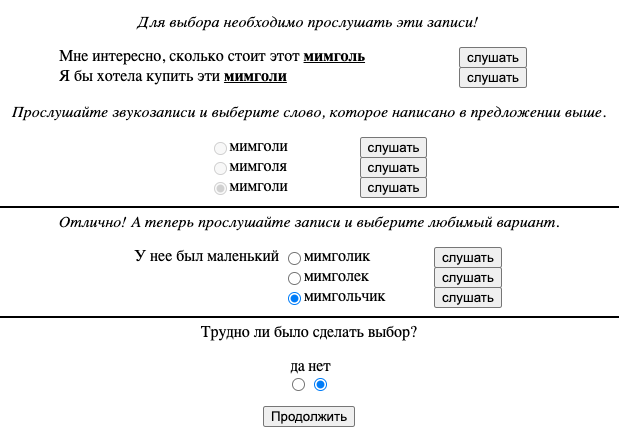
\includegraphics[width=\textwidth]{trial_ex.png}
 \caption{Screenshot of completed trial for nonce word study; horizontal lines separate the stages in which trial material was revealed}
 \label{fig:rutest}
\end{figure}

\begin{figure}
 \fbox{\parbox{.97\textwidth}{
 \centering
 \emph{Please listen to these recordings before selecting!}\\[\baselineskip]
 
 \begin{tabular}{lll}
  I'm interested in the price of that \textbf{\underline{mimɡolʲ}} & \fbox{play} & [mʲɪmɡólʲ] \\
  I would like to buy those \textbf{\underline{mimɡolʲi}}. & \fbox{play} & [mʲɪmɡɐlʲí]
 \end{tabular}\\[\baselineskip]
 
 \emph{Listen to the audio recordings and select the word written in the sentence above.}\\[\baselineskip]
 
 \begin{tabular}{lll}
  \like{0} mimɡolʲi & \fbox{play} & [mʲɪmɡólʲɪ]\\
  \like{0} mimɡolʲa & \fbox{play} & [mʲɪmɡɐlʲá]\\
  \like{7} mimɡolʲi & \fbox{play} & [mʲɪmɡɐlʲí]\\
 \end{tabular}\\[.5\baselineskip-\fboxsep]
 }}\vspace{-.5\fboxsep}
 \fbox{\parbox{.97\textwidth}{
 \centering\hfill\\[.5\baselineskip-2\fboxsep]
 
 \emph{Correct! Now listen to the recordings and select your favorite variant.}\\[\baselineskip]
 
 \begin{tabular}{l @{\hspace{1em}} lll}
  She had a little & \like{0} mimɡolʲik & \fbox{play} & [mʲɪmɡólʲɪk]\\
  & \like{0} mimɡolʲok & \fbox{play} & [mʲɪmɡɐlʲók]\\
  & \like{7} mimɡolʲtʃik & \fbox{play} & [mʲɪmɡólʲtʃʲɪk]\\
 \end{tabular}\\[.5\baselineskip-\fboxsep]
 }}\vspace{-.5\fboxsep}
 \fbox{\parbox{.97\textwidth}{
 \centering\hfill\\[.5\baselineskip-2\fboxsep] 
 Was the choice difficult?\\
 
 \begin{tabular}{cc}
  yes & no\\
  \like{0} & \like{7}
 \end{tabular} 
 }}
 \caption{Translation and transcription of \figref{fig:rutest} (with phonetic transcriptions, including unstressed vowel reduction, of recordings next to the buttons that played them)}
 \label{fig:entest}
\end{figure}

\subsection{Analysis}
All trials were kept except those with the one nonce word ending in a cluster, leaving 4,509 trials. As with the corpus study, I fitted a mixed logistic regression predicting whether \ok{} was selected as the diminutive (vs.\ \ik{} and \chik) on a given trial using forward stepwise regression (see \sectref{sec:corpanal} for details). Potential predictors included four phonological factors from the corpus study (the place and manner of the final consonant and the height and rounding of its last vowel); the others (length, stress, and coda complexity) were constant across the stimuli. Of these, the vowel factors did not improve the model and were not added. The presented plural was encoded as a three-way factor with stressed \plsi{} (the baseline) compared to unstressed \pli{} and stressed \pla. % be consistent about stress mark on -i?
I also included three potential experimental factors: trial number, the position in which \ok{} was listed among the possible diminutives (which was random), and whether participants found the choice difficult. Of these, only position of \ok{} (dummy-coded with second position as the baseline) was added to the final model. The model also included random intercepts for participant and stimulus.

A by-participant random slope of plural suffix was also included as a potential factor; however, it caused convergence issues and was thus not added to the model in the forward stepwise regression. Adding this random slope to the model slightly but significantly improves it ($\chi^2=11.6$, $p=.041$) and only minimally changes the effect sizes, with no change to their significance. Accordingly, I present the model successfully fitted by forward stepwise regression without the random slope.

\subsection{Results}
\subsubsection{Descriptive summary}
\tabref{tab:expdesc} shows how often participants selected each diminutive for nonce words depending on the plural with which they were presented.
\begin{table}
\begin{tabular}{lS[table-format = 3.0]S[table-format = 3.0]S[table-format = 3.0]S[table-format = 2.1{\tabpct}]<{{\tabpct}}}
\lsptoprule
\multicolumn{1}{l}{Plural} & {\chik} & {\ik} & {\ok} & \multicolumn{1}{c}{\unit{\percent} \ok}\\
\midrule
unstressed \pli & 573 & 547 & 570 & 33.7\\
stressed \plsi & 461 & 456 & 780 & 46.0\\
stressed \pla & 269 & 284 & 569 & 50.7\\
\lspbottomrule
\end{tabular}
\caption{Experimental frequency of selected diminutives by presented plural} % fix
\label{tab:expdesc}
\end{table}
For nouns with unstressed plural \pli, the diminutives were chosen with equal frequency. Participants chose \ok{} substantially more frequently for nouns with stressed \plsi{} (while \ik{} and \chik{} were chosen at equal rates), while \pla{} nouns had an even slightly higher rate of \ok{} (as well as a somewhat higher rate for \ik{} than \chik).

\subsubsection{Regression model}\label{sec:expmod}
As \tabref{tab:expmod} shows, the experimental effect of plural is significant, even when other factors are taken into account: plural \pla{} conditioned selection of \ok{} more frequently than plural stressed \plsi, which in turn saw significantly more use of \ok{} than its unstressed counterpart.
\begin{table}
\begin{tabular}{l@{~~}l@{~~}l@{}S@{~~~}S[table-format = 0.2, print-zero-integer = false]@{~~~}S@{~~~}S[table-format = +0.4, print-zero-integer = false]@{~}l}
\lsptoprule
\multicolumn{3}{l}{Effect} & {Estimate} & {SE} & {$z$ value} & {$p$ value}\\
\midrule
\multicolumn{3}{l}{Intercept} & -.17 & .22 & -.78 & .4373\\
\multicolumn{8}{l}{Plural}\\ % (default: coronal)}\\
& unstressed \pli & (vs.\ stressed \plsi) & -.65 & .08 & -8.20 & <.0001 & ***\\
& stressed \pla & (vs.\ stressed \plsi) & .23 & .09 & 2.71 & .0067 & **\\
\multicolumn{8}{l}{C place}\\ % (default: coronal)}\\
& labial & (vs.\ coronal) & -.32 & .21 & -1.51 & .1314\\
& dorsal & (vs.\ coronal) & .99 & .21 & 4.82 & <.0001 & ***\\
\multicolumn{3}{l}{Position of \ok{}}\\
& first & (vs.\ second) & .39 & .08 & 4.63 & <.0001 & ***\\
& third & (vs.\ second) & -.19 & .09 & -2.23 & .0258 & *\\
\multicolumn{8}{l}{C Manner}\\ % (default: plosive)}\\
& affricate & (vs.\ plosive) & 1.13 & .64 & 1.75 & .0797\\
& fricative & (vs.\ plosive) & -.28 & .20 & -1.43 & .1536\\
& nasal & (vs.\ plosive) & -.53 & .23 & -2.25 & .0248 & *\\
& approximant & (vs.\ plosive) & -.40 & .24 & -1.65 & .0992\\
\lspbottomrule
\end{tabular}
\caption{Fixed effects of mixed regression model predicting whether diminutive [ók] was selected in an experimental trial} % fix!
\label{tab:expmod}
\end{table}
The phonological shape of the stimuli also had a significant effect: nouns ending in dorsals were assigned \ok{} significantly more often than those ending in coronals, and nouns ending in nasals were given \ok{} significantly less often than nouns ending in plosives. The order in which the diminutive options were presented made a difference as well: the higher the diminutive with \ok{} was listed among the three options, the more often participants selected it. This model has $R^2=.230$. Multicollinearity between the factors is not problematic: the two phonological factors have a variance inflation factor (VIF) of $2.31$, while the others have a VIF of $1$ and $1.01$. % Speakers varied somewhat in their use of \ok{} (the random effect of speaker had a variance of $.39$), and individual nonce words also had some small differences as well (the random effect of stimulus had a variance of $.26$).

\subsubsection{Individual differences}
Individual participants varied in the rate at which they selected \ok{} compared to the other diminutive suffixes (minimum $4$, maximum $30$, mean $17$, standard deviation $5.7$).\footnote{All calculations in this section include trials with the nonce word removed from the main analysis for ending in a cluster, so that each individual has the same number of trials.} However, individuals' rates of \ok{} appear to be distributed normally: an asymptotic one-sample Kolmogorov-Smirnov test \citep{Massey1951} shows no significant difference between the distribution of individual \ok{} rates and a normal distribution. The same is true for the sizes of the plural effect, measured as the difference in an individual's rate of \ok{} for words with stressed plural \plsi{} vs.\ word with unstressed plural \pli{} and stressed plural \pla, respectively. Thus, I do not find evidence of any systematic difference in populations among participants.

Participants' country of origin also does not seem to have any detectable effect on the results. A factor comparing participants born in Russia (51 participants) to those born in Latvia (26), Ukraine (9), Lithuania (4), and elsewhere (24) does not yield any significant main effects or interactions with plural when added to the model presented in \sectref{sec:expmod}.

\subsection{Discussion}
The nonce word study shows that Russian speakers are sensitive to correlations between morphological patterns in their lexicon: they assigned \ok{} more often to nouns presented with a stressed plural suffix (matching the preference for \ok{} among nouns with suffix or mobile stress in the lexicon), and even more often when this plural suffix was \pla{}. The distribution of diminutives in the nonce word study was less extreme than in the lexicon, as is sometimes the case in such studies -- \citet{Ernestus.Baayen2003} and \citet{Zuraw2010} showed a narrower difference between the rate of (morpho)phonological alternation of different consonants in their nonce word studies than in their corpus studies. This narrowing may have several sources. First, my representation of the Russian language used in the corpus study in \sectref{sec:corp} is probably slightly different from the actual language input of my study's participants (in part because, as described in \sectref{sec:corpdata}, the Russian National Corpus represents the written standard). Second, speakers may be systematically reducing the rate of less common processes relative to their lexicon \citep[see][]{Hughto.etal2019}. Finally, these weaker results may reflect random noise: in some percentage of trials, participants were probably not paying attention. Regardless of which of these three factors (or a combination thereof) is correct, the important takeaway is that some effect was found: speakers are, to some degree, applying the hypothesized correlations.

Among the phonological factors tested, the final consonant influenced participants' choice of diminutive: nouns ending in dorsals were more likely to take \ok{} -- as in the lexicon and the nonce word experiment of \citet{Gouskova.etal2015} -- while nouns ending in nasals were less likely. This latter effect was significant in the corpus study of \citet{Gouskova.etal2015}, while my corpus study showed a non-significant effect in the opposite direction. Thus, their study more accurately represented speakers' input of the nasal effect (see \sectref{sec:corpdisc} for a discussion of the differences between the two corpus studies). The other phonological effect found in the corpus (word-final affricates condition lower rates of \ok{} than plosives) was not significant here, and the direction of the effect is opposite (however, as discussed in \sectref{sec:expstim}, only one stimulus, [xakóts], ended in an affricate). The factors for the last-syllable vowel, which were significant in the corpus study, did not make it into the model in \tabref{tab:expmod}.

Previous nonce word studies \citep{Gouskova.etal2015,Magomedova2017} find that \ok{} is somewhat less productive than the other two. However, in the present study, speakers did not seem to avoid \ok, and even preferred it in certain configurations. It may well be that these previous studies underrepresented the factors with which \ok{} is associated -- in particular, inflectional factors that cannot be inferred from the base form, which is what previous studies presented. As noted in \sectref{sec:corpdisc}, these inflectional properties are themselves less productive, leading to a conclusion that Russian speakers are perfectly happy to productively extend \ok{} to new words, but especially within classes that are themselves relatively closed.

% productivity

\section{General discussion}\label{sec:disc}
The nonce word study demonstrates that Russian speakers have learned two productive gradient correlations: masculine nouns with some or all stressed suffixes tend to take the diminutive \ok{}, and this tendency is even stronger if these stressed suffixes include the nominative plural \pla. Speakers use these generalizations productively when choosing a diminutive for new words. That is, this is part of speakers' morphological knowledge, and must be accounted for. In this section I propose that this knowledge is stored in the form of gradient constraints on the shape of underlying forms (morpheme structure constraints). In particular, I argue that the correlations between the three inflectional properties must be captured as correlations between three different pieces of underlying structure; plural and diminutive selection cannot be coindexed to the same inflectional marker. I discuss the implications of this conclusion for morphological theory.

\subsection{Formal analysis}\label{sec:fanal}
We are interested in the relationship between three morphological properties: stress pattern, plural allomorphy, and diminutive allomorph. How is each represented? As described in \sectref{sec:strbg}, nouns with fixed stem stress are typically analyzed as having underlying lexical accent on the stressed syllable (e.g.\ /avtóbus/), fixed suffix stress can be analyzed as a floating lexical accent (e.g.\ /karandaʂ´/), and mobile-stress nouns are underlyingly accentless (e.g.\ /volos/).

In \sectref{sec:plbg}, I noted that masculine nouns with plural \pla{}, which almost always have mobile stress in that they have stem stress in the singular and suffix stress in the plural, cannot all be analyzed as underlyingly accentless because the stem stress can fall on medial syllables (as in [utʃʲítʲelʲ] `teacher', whose plural is [utʃʲitʲelʲá]), whereas Russian phonology predicts that mobile-stress nouns should have stress on the first syllable in the singular. Thus, they may have a different underlying accent than mobile nouns with plural \pli. We will leave this problem aside and focus on the fact that these nouns select a different plural allomorph than most nouns of their inflectional macroclass.\footnote{One possibility, inspired by \citet{Matushansky2024}, is that plural \pla{} nouns take a plural suffix that is segmentally empty but accentually dominant, meaning that it erases any stress on its base. Thus, such nouns would behave as though accentless in the plural, meaning that the plural suffixes, which are underlyingly accented (including nominative /á/), would be stressed.} Since these nouns do not seem to differ syntactically from normal masculine nouns \citep{Matushansky2025}, I assume that they bear an inflection class feature, \feat{pl-a}, which resides in their phonological underlying form \citep{Harley.TubinoBlanco2013,Gouskova.Bobaljik2022,Tabachnick2023}: % cite pages lol
\urfeat{utʃʲítʲelʲ}{pl-a}.

Similarly, a noun's choice of diminutive must be memorized (for many nouns, at least). This, too, is typical behavior of arbitrary selection handled by diacritic features \feat{ok}, \feat{ik}, and \feat{chik} -- since the diminutive of [román] `novel' is [romántʃʲik], its underlying form is \urfeat{román}{chik}; the underlying form of [pósox] `staff', whose diminutive is [posoʂók], is \urfeat{pósox}{ok}. Since \ok{} diminutives have fixed suffix stress and are stress-dominant (erase any stress marks on their base), the underlying form is \urfeat[]{\underline{o}k´}{$+$dominant}, where /\underline{o}/ represents the fleeting vowel that disappears upon further suffixation and [$+$dominant] tags affixes that show stress dominance (see \sectref{sec:dimbg}; the exact phonology of these two properties is not relevant).

\subsection{Correlations between pieces of underlying structure}\label{sec:coranal}
I propose that speakers have learned generalizations of varying strengths that determine the well-formedness of underlying forms -- in essence, gradient morpheme structure constraints \citep[see][]{Booij2011} -- represented formally in \REF{ex:consts}:
\ea\label{ex:consts} \emph{Russian gradient morpheme structure constraints}\\
    \ea\label{ex:constsyll} *σ́, \feat{ok}
    \ex\label{ex:constpd} \feat{pl-a} $\rightarrow$ \feat{ok}
    \z
\z
The first constraint, \REF{ex:constsyll}, is a cooccurrence restriction violated by underlying forms that contain both an accented syllable and the diacritic feature \feat{ok}.\footnote{This restriction is presented as non-local; however, if -- as assumed by e.g.\ \citet[][374]{Chomsky.Halle1968} -- diacritic features are distributed to every segment of a lexical item, \REF{ex:constsyll} can be represented as a local cooccurrence restriction.} Given that fixed stem stress is represented by lexical accent on a syllable, \REF{ex:constsyll} captures the fact that nouns with stem stress are substantially underrepresented among words that take \ok{} relative to words with suffix or mobile stress. Since such nouns do still appear with some frequency, however, this constraint would not be overwhelmingly strong. % lay out what ``strength'' means?

The second constraint, \REF{ex:constpd}, is an implicational relationship between two diacritic features \citep[cf.][]{Halle.Marantz2008}: lexical items that have the \feat{pl-a} feature (indexing plural \pla) must also have the \feat{ok} feature (indexing diminutive \ok).\footnote{Since the \feat{ok}, \feat{chik}, and \feat{ik} features are essentially complementary, \REF{ex:constpd} can be replaced by two cooccurrence restrictions penalizing plural \pla{} nouns with other diminutives: *\feat{pl-a}, \feat{ik} and *\feat{pl-a}, \feat{chik}. This is theoretically desirable under approaches \citep[e.g.][]{Hayes.Wilson2008} that require constraints to penalize the presence of structure -- that is, be framed negatively.} % cite
The relationship between these two features in the lexicon is rather strong, but some of this correlation can be attributed to stress pattern rather than the \feat{pl-a} feature; the experimental effect of plural \pla{} over stressed \plsi{} was fairly weak.

The constraints in \REF{ex:consts} are \emph{not} a part of the generative grammar; they are not invoked in the course of a normal derivation. Instead, as well-formedness constraints on underlying forms, they are invoked when necessary to ``fill in'' an underlying form \citep[cf.][]{Gouskova.etal2015} that is lacking crucial information, as in the case of nonce words. % PCFP
The task of choosing a diminutive for a novel word (or any word for which a speaker has no stored diminutive) is as follows. I assume that abstract syntactic objects like a diminutive head are spelled out phonologically using rules of realization, as in Distributed Morphology \citep[see e.g.][]{Halle.Marantz1993,Harley.Noyer1999,Steriopolo2008}. The Russian speaker's set of realization rules includes (among others) the three possibilities for the diminutive in \REF{ex:dimvis} and two for the plural in \REF{ex:plvis} (the latter of which are considerably oversimplified in ways that are not relevant here):\footnote{In contexts with \feat{pl-a}, the more specific rule in \REF{ex:avi} wins over the generic rule in \REF{ex:ivi} according to the Subset Principle \citep{Halle1997b}. In other contexts, the default \REF{ex:ivi} wins.}

\ea\label{ex:dimvis} \emph{Rules of realization for the Russian diminutive}\\
    \ea\label{ex:okvi} \DIM{} $\rightarrow$ \underline{o}k´\textsubscript{[$+$dominant]} / \feat{ok}\gap
    \ex\label{ex:ikvi} \DIM{} $\rightarrow$ ʲik\hspace{\widthof{ok´\textsubscript{[$+$dominant]}}-\widthof{ʲik}} / \feat{ik}\gap
    \ex\label{ex:chikvi} \DIM{} $\rightarrow$ tʃʲik\hspace{\widthof{ok´\textsubscript{[$+$dominant]}}-\widthof{tʃʲik}} / \feat{chik}\gap
    \z
\ex\label{ex:plvis} \emph{Rules of realization for the Russian plural (oversimplified)}\\
    \ea\label{ex:avi} \NOM{} \PL{} $\rightarrow$ a / \feat{pl-a}\gap
    \ex\label{ex:ivi} \NOM{} \PL{} $\rightarrow$ i
    \z
\z
The rules in \REF{ex:dimvis} insert each of the three diminutives in the context of its corresponding diacritic feature, which is brought into the derivation by the noun stem. Thus, the diminutive will be spelled out as /tʃʲik/ in the context of \urfeat{román}{chik} because the \feat{chik} feature matches the structural conditions for rule \REF{ex:chikvi}. If a noun does not have one of the three features, none of the rules in \REF{ex:dimvis} can apply. This, of course, is the situation with nonce words, for which speakers have not previously seen a diminutive and thus cannot have a stored selectional preference. Thus, if they wish to assign a diminutive to a noun, they must place one of the diminutive features on its lexical item.

How do speakers determine which of \feat{ok}, \feat{ik}, or \feat{chik} to assign to their noun? I argue that, essentially, they throw a weighted die \citep[see e.g.][]{Albright.Hayes2003,Ernestus.Baayen2003,Hayes.etal2009}: % and more?
each of the three possible options is assigned a ``well-formedness'' score, and the better a feature for a given underlying form, the more likely it is to be assigned. The well-formedness score is assigned by gradient, weighted constraints, including those in \REF{ex:consts}. Of course, by this point the speaker does already have an underlying form for the nonce word inferred from the singular and plural, as shown in \tabref{tab:nonceurs}.
\begin{table}
\begin{tabular}{lll}
\lsptoprule
Singular & Plural & Underlying form\\
\midrule
{[mʲimɡólʲ]} & [mʲimɡólʲi] & /mʲimɡólʲ/\\
{[mʲimɡólʲ]} & [mʲimɡolʲí] & /mʲimɡolʲ´/\\
{[mʲimɡólʲ]} & [mʲimɡolʲá] & \urfeat{mʲimɡolʲ´}{pl-a}, \urfeat{mʲimɡólʲ}{pl-a}\\
\lspbottomrule
\end{tabular}
\caption{Possible underlying forms for the nonce word [mʲimɡólʲ] given observed singular and plural forms}
\label{tab:nonceurs}
\end{table}
This table shows how a word's singular and plural indirectly affect its likely diminutive. If a word is shown with unstressed plural \pli, it must have fixed stem stress and thus underlying lexical accent on the syllable. Assigning \feat{ok} to this word would violate \REF{ex:constsyll}, so the likelihood of doing so will be lower than for words without an underlying accented syllable. Nouns with stressed plural \plsi{} must have suffix stress, and thus get a floating stress mark; assigning \feat{ok} to such words would not be penalized by \REF{ex:constsyll}. If a noun has plural \pla, it gets the \feat{pl-a} feature, so assigning anything other than \feat{ok} to this word (i.e., \feat{ik} or \feat{chik}) would be heavily penalized by \REF{ex:constpd}. Thus, words with \feat{pl-a} are more likely than others to get \feat{ok}. Since nouns with plural \pla{} can have different stress patterns in their singular and plural (see \sectref{sec:fanal}), the nominative singular and plural alone are compatible with two stress patterns in the singular: fixed suffix stress, with floating underlying accent (which would fall on the last syllable of the stem in the unsuffixed nominative), and fixed stem stress, with linked underlying accent -- these nonce words cannot be mobile stress nouns, because in that case they would have the first syllable stressed in the nominative singular. If speakers represent these nouns as having fixed suffix stress, assigning \feat{ok} to them would violate \REF{ex:constsyll}; this may be one reason why the experimental effect of plural \pla{} was relatively small.

The well-formedness constraints proposed here are similar to those capturing phonological tendencies in diminutive selection described by \citet{Gouskova.etal2015} -- % and others
for example, the strong preference for nouns ending in dorsals to take \feat{ok} both in the lexicon and experimentally is instantiated by a constraint penalizing word-final dorsals, *[+low]\#, active for words that take \feat{ik} and \feat{chik}. However, their constraints are phonotactic in nature, evaluating surface forms of bases, whereas mine operate on underlying forms.

\subsection{Alternative: unified representation}\label{sec:alt}
In the analysis presented above, a word's morphological properties are divided up into three distinct pieces of representation, one phonological (underlying accent marking inflectional stress) and two diacritic (marking plural, in the case of \pla, and diminutive selection).\footnote{In the analysis in \sectref{sec:coranal}, these diacritic markers are also phonological in the sense that they reside in the phonological underlying form. However, they do not use the vocabulary of the phonological module.} In this section, I explore the possibility of unifying plural and diminutive allomorph selection under a single diacritic marker, concluding that such an analysis is inferior to that in \sectref{sec:coranal}.

% This, in turn, poses difficulties for attempts to eliminate diacritic markers from morphology by expressing the information they contain to phonological or syntactic representations. % put in better context and cite: Ora, Ulfsbjorninn, Nanosyntax, etc. - or expound at the end of this section

% More restrictive theories of the lexicon typically assume an approach with two levels of productivity: % cite
% certain inflectional patterns can be captured using the standard vocabulary of the phonological or syntactic module, and these are productive; those that cannot be thus captured are exceptions that are (depending on the analysis) stored in full, stored in special non-productive but still compositional forms (like the private lexical entries of Nanosyntax), % cite
% or simply ignored. No matter what the non-standard representation, they are generally taken to be unproductive. Thus, the question becomes: can a unified diacritic marker (or, equivalently, a unified non-diacritic representation) account for the productivity displayed by speakers in the nonce word study?

The motivation for this alternative analysis is the fact that nouns with plural \pla{} almost always take diminutive \ok. Linguists often analyze strong distributional correlations like this one as fully productive -- that is, encoded into the rules of the grammar. Under this approach, we ``hard-code'' the correlation into the rule in \REF{ex:okavia}: the same \feat{pl-a} feature that indexes plural \pla{} in \REF{ex:avi} is directly invoked in the spellout of \ok{}.
\ea\label{ex:okavia} \emph{Proposed additional rule of realization for the Russian diminutive}\\
    \DIM{} $\rightarrow$ \underline{o}k´\textsubscript{[$+$dominant]} / \feat{pl-a}\gap
\z
% \ea\label{ex:dimvias} \emph{Additional rules of realization for the Russian diminutive}\\
%     \ea\label{ex:okavia} \DIM{} $\rightarrow$ \underline{o}k´\textsubscript{[$+$dominant]} / \feat{pl-a}\gap
%     \ex\label{ex:ikavia} \DIM{} $\rightarrow$ ʲik\hspace{\widthof{ok´\textsubscript{[$+$dominant]}}-\widthof{ʲik}} / \feat{ik+pl-a\textrm{, }pl-a}\gap
%     \z
% \z
This move introduces two further issues. First, the \feat{ok} feature is still needed for the nouns with diminutive \ok{} and plural \pli{} (which far outnumber those with plural \pla). This feature is, as before, invoked in rule \REF{ex:okvi}; thus, two rules point to the same realization, \urfeat[]{\underline{o}k´}{$+$dominant} (or, alternatively, we combine them into a single rule with a disjoint context).
Second, we need an additional feature, \feat{ik+pl-a}, to override the association between \feat{pl-a} and diminutive \ok{}. This rule sits alongside \feat{pl-a} for those few words with plural \pla{} that take a different diminutive (\ik). Both features are then invoked in the diminutive spellout rule in \REF{ex:ikavia}:
\ea\label{ex:ikavia} \emph{Required additional rule of realization for the Russian diminutive}\\
    \DIM{} $\rightarrow$ ʲik / \feat{ik+pl-a\textrm{, }pl-a}\gap
\z
This rule duplicates spellout of /ʲik/ from the rule in \REF{ex:ikvi} just as the rule in \REF{ex:okavia} duplicates \REF{ex:okvi}.\footnote{These nouns must also have the \feat{pl-a} feature to match rule \REF{ex:avi} spelling out the plural as \pla. The rule in \REF{ex:ikavia} must then require both \feat{pl-a} and \feat{ik+pl-a} in order to be more specific than rule \REF{ex:okavia}, and thus win out by the Subset Principle \citep{Halle1997b} when both rules' conditions are met.}

% We can simplify this analysis slightly if we assume that diacritic features may be in an inheritance relation -- that is, \feat{pl-a} is a sub-feature of \feat{ok}, while \feat{ik+pl-a} is a sub-feature of \feat{ik}. In this case, the rules in \REF{ex:dimvias} are not necessary, since the \feat{pl-a} feature will count as an \feat{ok} feature in the context of the usual rule spelling out the diminutive as \ok{} in \REF{ex:okvi}. However, if diacritic features are, as proposed in this section, stand-ins for features or structures that properly use the phonological (or syntactic) vocabulary, it is difficult to see how this inheritance structure would work. % rework

Since nouns with plural \pla{} get \feat{pl-a}, rule \REF{ex:okavia} should apply by default to these words without the need for productive feature filling as described in \sectref{sec:coranal}. In this case, we should expect the effect size of plural \pla{} to be much greater in the nonce word study than it was: even accounting for some amount of random noise in the task effect, the use of \ok{} for nouns with plural \pla{} is predicted to be close to ceiling. In actuality, \ok{} was selected for nouns with \pla{} just over half the time -- only a moderately higher rate than for nouns with plural \pli.

% Alternately, speakers may (by some mechanism similar to that described in \sectref{sec:coranal}) choose proportionately between assigning \feat{pl-a} and \feat{ik+pl-a}. This predicts similar empirical results to the analysis in \sectref{sec:coranal}, although it more strongly predicts that nouns with plural \pla{} should never be assigned \chik{, since they are not in the lexicon; in the nonce word study, however, such words were assigned \ik{} and \chik{} at roughly equal rates.

In an attempt to reduce theoretical machinery, we have instead increased it, with one new feature, \feat{ik+pl-a}, and two new rules, in \REF{ex:okavia} and \REF{ex:ikavia}. Doing so also reduced our empirical coverage. Thus, plural and diminutive allomorph selection should remain \emph{formally distinct} and the correlation between them should be handled in a separate pattern-matching module.

This finding has implications for morphological theory. While the analysis presented here uses diacritic features, some linguists argue against the use of morphological diacritics on theoretical grounds, aiming to replace them either with complex stored stems \citep[e.g.][]{BermudezOtero2013} or pieces of phonological \citep[e.g.][]{Lampitelli.Ulfsbjorninn2023} or syntactic \citep[e.g.][]{Caha2021} structure. This section, then, shows that any analyses of Russian without diacritics must be flexible enough to satisfy the following two criteria: first, a noun's plural and diminutive selection are stored as \emph{separate} and \emph{independent} markers, and second, all three morphological markers must be accessible to pattern-matching mechanisms like the morpheme structure constraints proposed in \sectref{sec:coranal}.

Let us take one theory that rejects diacritics, Nanosyntax, as an example. In ``classical'' Nanosyntax \citep[e.g.][]{Caha2021}, lexical entries comprise one-dimensional stacks of functional heads that determine a word's inflectional paradigm, and having two suffixes vary independently is problematic. However, recent developments in the theory like complex left branches \citep{Blix2021}, exemplified in \citet{Janku2022} and \citet{Cortiula2023}, introduce greater complexity to lexical entries and likely provide them with enough flexibility to handle independence between the plural and diminutive. The second criterion remains problematic for Nanosyntax: plural and diminutive allomorphy would be encoded in syntactic structure, while inflectional stress pattern would be phonological, as described previously. Since the encodings of diminutive and stress pattern do not share a vocabulary and are separated by a modular wall, it is unclear how both could be included in a single morpheme structure constraint. Thus, this example emphasizes that a morphological theory must be able to accommodate not just a particular set of static paradigms deemed productive, but also psychologically real gradient generalizations.

\section{Conclusion}\label{sec:conc}
In this study, I provided corpus evidence for the influence of two inflectional properties on the choice of diminutive for Russian masculine nouns: inflectional stress pattern and plural suffix. Moreover, a nonce word study shows that speakers have learned these correlations from their lexicon and productively apply them. I argued that this correlation is not encoded into the structure of morphological markers in the lexicon, but rather emergent in a pattern-matching module productively drawing generalizations over underlying forms akin to morpheme structure constraints.

This work is important for theoretical morphology in several ways. First, it serves as a reminder that the lexicon is not enough: we need pattern matching as well. %, and linguists should be careful not to assume that all inflectional correlations are properties of a unified ``inflectional class''.
Second, it exemplifies the importance of addressing gradience and variation in the study of inflectional paradigms, as is common in the non-generative literature \citep[e.g.][]{Ackerman.Malouf2013} but often ignored in generative work on inflectional patterns (which often focuses on accounting for syncretisms). Finally, it sets a benchmark for approaches to morphology that wish to do away with diacritic markers, instead encoding all inflectional information within the regular vocabulary of phonology and/or syntax: these must be in multiple pieces (such that inflection class, plural selection, and diminutive selection are encoded separately) and accessible to the pattern-matching module (that is, arguably, they must all be in the \emph{same} module, presumably phonology). % evidence elsewhere

\section*{Abbreviations}

\begin{tabularx}{.5\textwidth}{@{}lQ}
\DAT &dative\\
\DIM &diminutive\\
\NOM &nominative\\
\end{tabularx}%
\begin{tabularx}{.5\textwidth}{lQ@{}}
\PL &plural\\
\SG &singular\\
&\\ % this dummy row achieves correct vertical alignment of both tables
\end{tabularx}

\section*{Acknowledgements}
Place your acknowledgements here and funding information here.
% DDRIG, IRB

%\section*{Contributions}
%John Doe contributed to conceptualization, methodology, and validation. 
%Jane Doe contributed to writing of the original draft, review, and editing.

\sloppy
\printbibliography[heading=subbibliography,notkeyword=this]
\end{document}
